\documentclass[10pt]{article}
\usepackage[margin=0.82in]{geometry}
\usepackage{amsmath,amssymb,booktabs,graphicx,microtype,float,placeins}
\usepackage[font=small,skip=3pt]{caption}
\usepackage[hidelinks]{hyperref}
\setlength{\parindent}{0pt}
\setlength{\parskip}{3pt plus 1pt minus 1pt}
\setlength{\textfloatsep}{7pt plus 2pt minus 2pt}
\setlength{\intextsep}{7pt plus 2pt minus 2pt}
\title{\vspace{-1.7em}\textbf{Where Major Theorems Live in Proof Space}\vspace{-0.5em}}
\author{J. R. Landers\\[-1pt]\small A controlled map against LeanDojo Benchmark 4}
\date{\vspace{-1.4em}}

\begin{document}
\maketitle
\vspace{-1.5em}

\begin{abstract}
We locate 18,852 Lean declarations from nine repositories containing major
recent formalizations in embedding spaces anchored by 10,000 frozen LeanDojo
theorem--proof pairs.  The repositories are peripheral: their raw mean
statement-density deficit is 0.0945 cosine points, and 62.7\% of declarations
fall below LeanDojo's own fifth density percentile.  A sequence of controls
changes the interpretation.  Length and coarse domain, exact toolchain date,
surface style, source architecture, dependency depth, and reusable compression
do not remove the shift.  Bound-name and conservatively resolved project-global
vocabulary ablations jointly reduce the exact-snapshot deficit by 46.3\%, from
0.0600 to 0.0322, but a significant repository-level residual remains.  Most
importantly, 34 named headline theorems are not more isolated than
same-repository, same-domain, architecture-matched declarations.  Thus the
observed rarity belongs primarily to repository dialect and mathematical
ecology, not specifically to celebrated endpoints.  Embedding rarity alone is
therefore not evidence of theorem-level creativity.
\end{abstract}

\paragraph{Corpus and estimand.}
The fixed reference set $R$ contains 10,000 seed-0 LeanDojo declarations.  The
frontier corpus contains OpenAI's Ten Proofs and Navier--Stokes/Euler projects,
FLT, PFR, PNT+, Formalized Formal Logic, Jordan--Sch\"onflies, Liquid Tensor,
and Sphere Eversion.  Large repositories contribute a seed-0 sample of about
2,500 declarations plus all identified headline theorems; smaller projects are
retained in full.  There are 18,852 declarations and 36 named endpoints, of
which 34 in eight Lean 4 projects enter the controlled headline analysis.

For unit-normalized statement embedding $z_t\in\mathbb R^{1024}$, define
reference-neighborhood density
\[
 \rho_k(t)=\frac1k\sum_{r\in N_k(t)}\langle z_t,z_r\rangle,
 \qquad
 N_k(t)=\operatorname*{arg\,topk}_{r\in R}\langle z_t,z_r\rangle .
\]
Low $\rho_k$ means that $t$ is locally rare relative to the frozen reference.
For each frontier declaration $t$, let $m(t)$ be an exact-snapshot Mathlib
control matched on frozen raw semantic cluster and statement length.  Its
positive isolation residual is
\[
 A(t)=\rho_k(m(t))-\rho_k(t).
 \tag{1}
\]
Project means, rather than thousands of declarations, are the replication
units for reported intervals.  For an ablated representation $a$, define
attenuation of a negative matched gap $\Delta$ by
\[
 \eta_a=1-\frac{|\Delta_a|}{|\Delta_{\rm raw}|}.
 \tag{2}
\]

\paragraph{Initial map.}
In the original frozen map at $k=10$, mean frontier statement density is
0.6717 versus 0.7662 within LeanDojo; proof density is 0.7030 versus 0.7971.
Accordingly, 62.7\% of frontier statements and 60.7\% of frontier proofs lie
below the corresponding LeanDojo fifth-percentile thresholds.  Semantic
neighbors are still useful: statements selected as neighbors have proofs 0.0565
cosine points closer to the frontier proof than random reference proofs.  The
corpora are peripheral, not detached.  Figure~\ref{fig:spaces} displays the
same project clouds in statement and proof views.

\begin{figure}[!htbp]
  \centering
  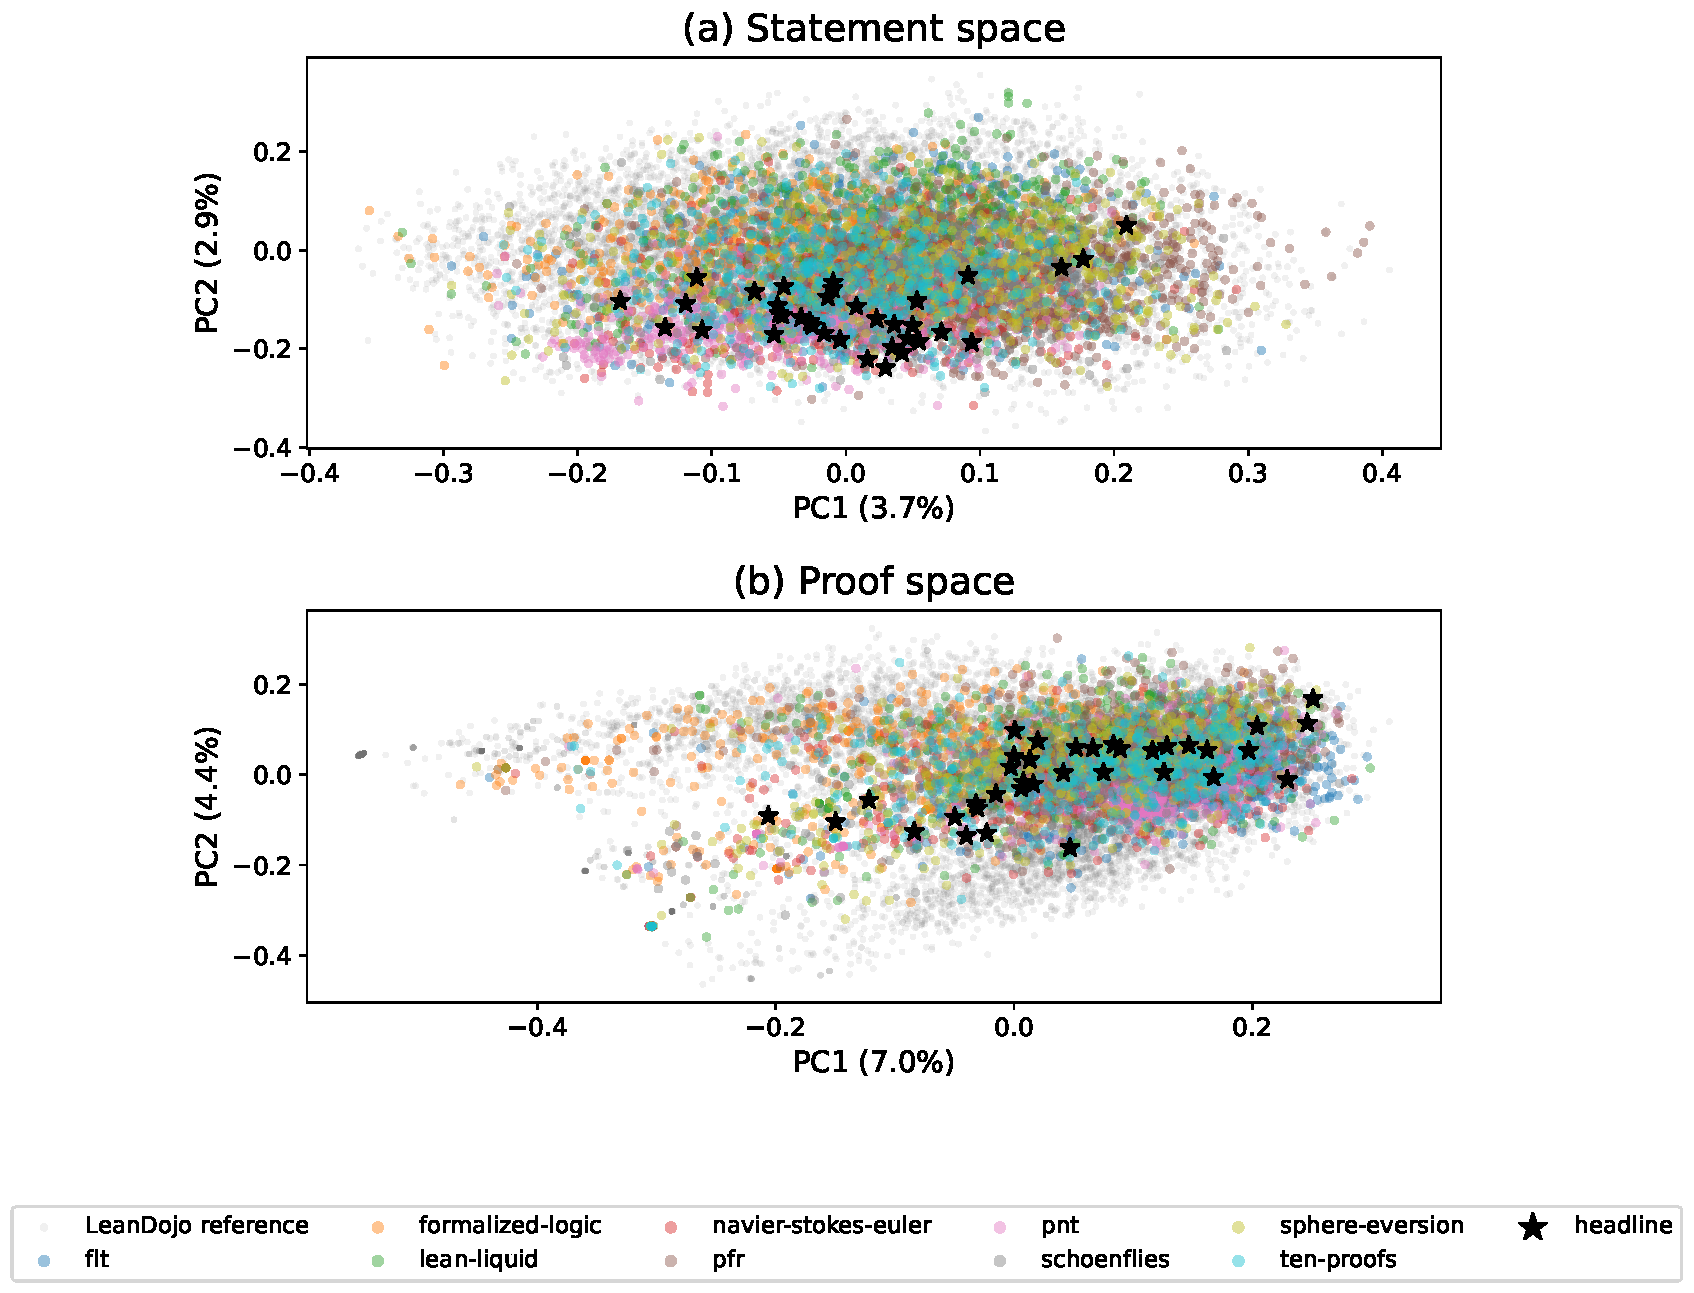
\includegraphics[width=0.94\textwidth]{../../experiments/frontier-formalizations/figures/frontier_spaces_dual.pdf}
  \caption{Statement (top) and proof (bottom) embeddings in separate 2D PCA
  bases fitted only on the corresponding LeanDojo reference (gray).  Colors
  identify repositories and stars mark headline declarations.  The displaced
  clouds establish repository-level distribution shift; they do not show that
  headline stars are exceptional within their own clouds.  Statistics use the
  full 1,024-dimensional vectors, not these projections.}
  \label{fig:spaces}
\end{figure}
\FloatBarrier

\paragraph{What explains the displacement?}
Table~\ref{tab:controls} summarizes the successive tests.  Length plus frozen
coarse semantic cluster explains about 22\% of the initial shift.  Replacing
the old reference comparison with 21,000 declarations from the projects'
exact pinned Mathlib snapshots leaves a raw project-balanced gap of $-0.0600$.
Removing headers does not reduce it.  Alpha-normalizing local bound names
reduces it to $-0.0452$.  Static source architecture is not a robust
explanation: a linear adjustment gives $-0.0338$, whereas a cross-fitted random
forest gives $-0.0445$.  The conclusion depends on model specification rather
than revealing a stable mechanism.

\begin{table}[!htbp]
\centering
\small
\begin{tabular}{p{0.34\textwidth}rrp{0.30\textwidth}}
\toprule
Test & Effect & 95\% project interval & Interpretation \\
\midrule
Raw exact-snapshot match & $-0.0600$ & $[-0.0791,-0.0409]$ & Recency and toolchain drift do not remove the gap. \\
Headers removed & $-0.0625$ & $[-0.0840,-0.0410]$ & Declaration headers are not the cause. \\
Bound names also removed & $-0.0452$ & $[-0.0685,-0.0220]$ & Local naming explains 24.6\% of the raw gap. \\
Static architecture, linear & $-0.0338$ & $[-0.0596,-0.0080]$ & Suggests attenuation, but is model-sensitive. \\
Static architecture, nonlinear & $-0.0445$ & $[-0.0656,-0.0235]$ & Only 1.5\% attenuation; architecture is not robust. \\
Project globals anonymized & $-0.0322$ & $[-0.0508,-0.0136]$ & 28.8\% beyond bound names; 46.3\% total attenuation. \\
\bottomrule
\end{tabular}
\caption{Matched frontier-minus-control density effects.  Negative values mean
frontier declarations remain less dense.  The ablations identify sensitivity
to representation, not causal shares, and their percentages should not be
added except along the stated nested raw $\rightarrow$ bound-name
$\rightarrow$ project-vocabulary sequence.}
\label{tab:controls}
\end{table}

The vocabulary test starts from alpha-normalized statements and replaces
lexically resolved project-defined global constants by statement-local
placeholders $g_0,g_1,\ldots$, preserving repeated-symbol identity and Mathlib
vocabulary.  Resolution is deliberately conservative: exact qualified names
are replaced, while ambiguous unqualified names are retained.  It changes
10,269 of 18,852 statements and 22,527 symbol occurrences.  The remaining
$-0.0322$ gap is significant, so spelling and repository API alone are
insufficient.  Figure~\ref{fig:ablations}(a) shows strong heterogeneity:
Formalized Logic and Sphere Eversion approach the reference, whereas PNT+,
Navier--Stokes, Ten Proofs, and Sch\"onflies remain displaced.

\paragraph{Dependency geometry.}
Let $G=(V,E)$ be a source-static dependency graph with $t\to u$ when the body
of $t$ lexically names declaration $u$.  The graph contains 825,962
declarations and 5,009,790 resolved edges.  Define the prerequisite cone and
synthesis depth
\[
 P(t)=\{u:t\leadsto u\},\qquad
 D(t)=\max_{u\in P(t)}\operatorname{dist}_G(t,u).
 \tag{3}
\]
For prerequisite $u$, with direct downstream reuse $r(u)$, body length
$|p_u|$, and name length $|n_u|$, define a source-level shortcut saving
\[
 S(u)=\max\{0,(r(u)-1)|p_u|-r(u)|n_u|\},\qquad
 C(t)=\frac{\sum_{u\in P(t)}S(u)}
 {\sum_{u\in P(t)}S(u)+\sum_{u\in P(t)}|p_u|}.
 \tag{4}
\]
Excluding macro-obscured FLT, headline cones are an estimated 2.25 dependency
steps deeper than matched declarations (interval $[0.01,4.48]$), but their
compression-fraction lift is $-0.026$ ($[-0.098,0.046]$).  More importantly,
across 16,350 declarations the controlled association between one standard
deviation of $\log(1+D)$ and isolation residual is only 0.0014
($[-0.0019,0.0047]$).  Depth plus compression add 0.32\% five-fold
out-of-sample explained variance ($[-0.08\%,0.73\%]$).  Deeper synthesis may
describe some endpoints, but it does not explain the semantic displacement.

\paragraph{Are the major theorems themselves rare?}
This is the decisive distinction.  For headline $h$, let $M_P(h)$ contain up
to 20 non-headline declarations from the same repository and raw semantic
cluster, nearest in statement/proof length, file position and size, scope,
binders, imports, and local-reference features.  Define
\[
 H(h)=\frac1{|M_P(h)|}\sum_{c\in M_P(h)}\rho_k(c)-\rho_k(h).
 \tag{5}
\]
Positive $H$ means that a headline is more isolated than comparable local
work.  Across 34 modern headlines, the project-balanced mean is $-0.0060$
($[-0.0252,0.0133]$).  After excluding 5,492 sampled declarations in any
headline prerequisite cone, it is $-0.0020$ ($[-0.0235,0.0195]$).  Excluding
FLT's macro-wrapped endpoints gives 0.0049 ($[-0.0116,0.0215]$).  None differs
from zero.  Most exact-cluster matches use 20 controls; one sparse PFR cell has
two, and matching balance is imperfect, but all specifications give the same
null conclusion.  Figure~\ref{fig:ablations}(b) shows the project effects.

\begin{figure}[!htbp]
  \centering
  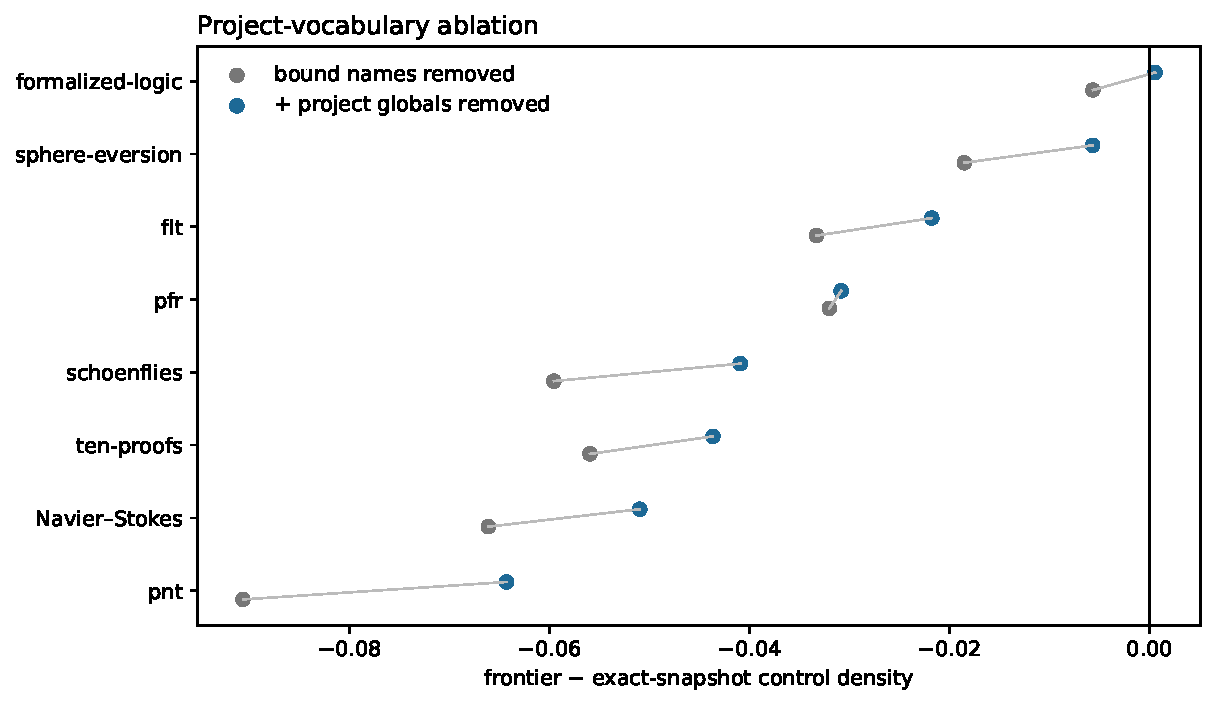
\includegraphics[width=0.78\textwidth]{../../experiments/frontier-vocabulary-ablation/figures/vocabulary_ablation.pdf}
  \vspace{2pt}

  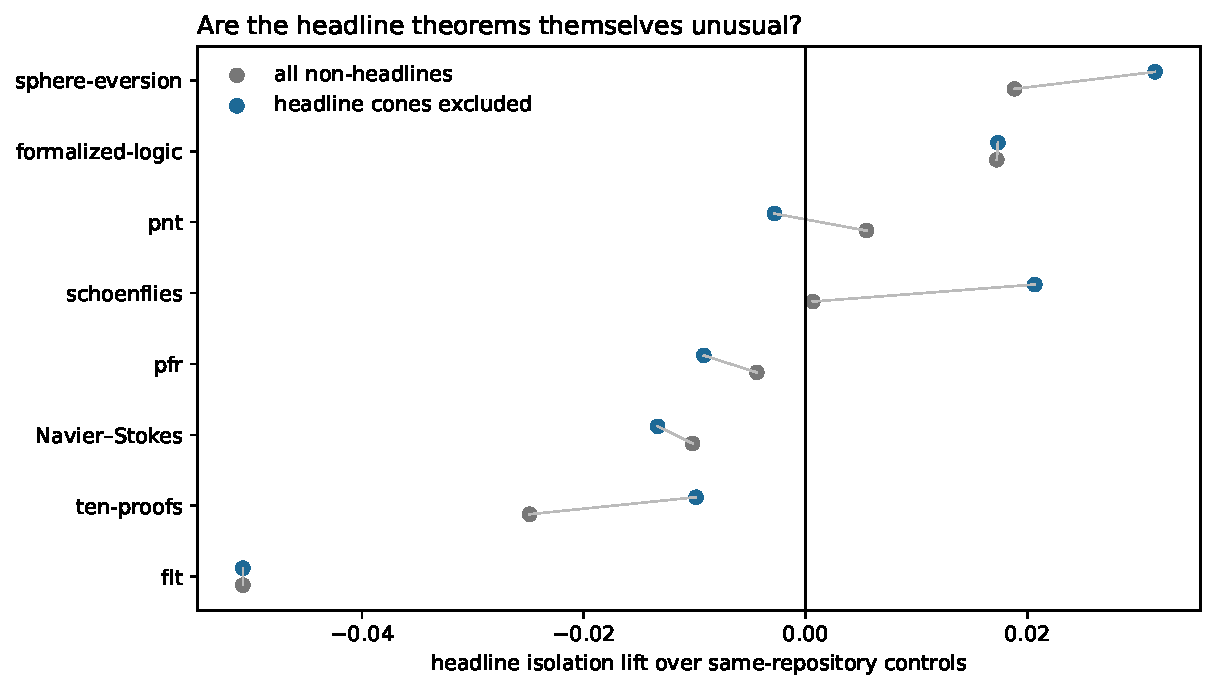
\includegraphics[width=0.78\textwidth]{../../experiments/frontier-headline-isolation/figures/headline_isolation.pdf}
  \caption{Two tests of what the original project clouds mean.  (a) Removing
  conservatively resolved project-global vocabulary moves every project toward
  the exact-snapshot reference, but several gaps remain.  (b) Within those
  repositories, named headline theorems are not consistently more isolated
  than same-domain architecture-matched declarations; positive values would
  indicate headline-specific rarity.}
  \label{fig:ablations}
\end{figure}
\FloatBarrier

\paragraph{Creativity formalism.}
The motivating triad is
\[
 \mathcal K(t)=
 \underbrace{\mathcal S(t)}_{\text{structure preservation}}
 \;\times\;
 \underbrace{\mathcal G(t)}_{\text{compression gain}}
 \;\times\;
 \underbrace{\mathcal R(t)}_{\text{low prior probability}}.
 \tag{6}
\]
The product notation emphasizes that rarity alone is insufficient.  For a Lean
proof, type checking supplies strong evidence for $\mathcal S$.  Embedding
isolation is at best a proxy for $\mathcal R$ under the explicitly chosen
LeanDojo prior.  Equations (3)--(4) test limited source-level proxies for
$\mathcal G$; they do not measure conceptual explanatory compression.

The experiments establish repository-level rarity
$\mathcal R(\text{project}\mid\text{LeanDojo})$, partly induced by vocabulary.
They do \emph{not} establish conditional headline rarity
$\mathcal R(h\mid\text{project})$, because (5) is null, nor do they establish
compression gain.  Consequently the current map cannot support a claim of
theorem-level creativity.  A suitable next target is explanatory compression:
whether a new abstraction shortens many derivations, generates unusually many
nontrivial consequences, or joins previously weakly connected mathematical
modules while preserving correctness.

\paragraph{Conclusion and limits.}
Where do major theorems live?  Repositories containing them live near the edge
of the frozen LeanDojo space.  The named endpoints themselves do not occupy a
detectably more peripheral region than comparable declarations in those same
repositories.  Roughly 46\% of the controlled displacement is sensitive to
local and project-global naming; the residual is best described as
repository-level mathematical-content and representation shift, not
``profoundness.''

The remaining limitations are substantive.  Embeddings measure textual
representation rather than mathematical equivalence.  Global-symbol
anonymization and dependency resolution are lexical, FLT hides structure behind
proof macros, exact-cluster control cells can be sparse, and eight projects are
few independent replication units.  Elaborated dependencies and a direct
measure of consequence-level compression are required before revisiting the
creativity hypothesis.

\paragraph{Reproducibility.}
Frozen commits, inputs, sampling, controls, code, figures, and machine-readable
results are retained under \texttt{experiments/frontier-*}.  The final
vocabulary ablation re-embedded only frontier statements, reused prior
reference/control vectors, and cost an estimated \$0.162.  All experiments
remained below the precommitted \$15 AWS cap.

\end{document}
